\documentclass[12pt, a4paper, titlepage]{article}
\usepackage[ngerman]{babel}
\usepackage{csquotes}
\usepackage{color}
% \usepackage[doi=false,isbn=false,citestyle=verbose,bibstyle=numeric,sorting=nty, backend=biber]{biblatex}

\usepackage[doi=false, isbn=false, style=verbose,sorting=nty, backend=biber]{biblatex}
\renewcommand*{\labelnamepunct}{\addcolon\space} % add : between author and title
\renewbibmacro*{in:}{\space In:}
\DeclareFieldFormat*{title}{\mkbibquote{#1}\nopunct}
\DeclareFieldFormat*{number}{{#1}\adddot\nopunct}
\renewbibmacro*{journal+issuetitle}{%
  \usebibmacro{journal}%
  \setunit*{\addspace}%
  \iffieldundef{series}
    {}
    {\newunit
     \printfield{series}%
     \setunit{\addspace}}%
  \setunit{\addspace}%
  \renewbibmacro{volume+number+eid}{
	  \printfield{volume}
  }
  \usebibmacro{volume+number+eid}
  \usebibmacro{issue+date}%
  \setunit{\addcolon\space}%
  \usebibmacro{issue}%
  \setunit{H. }%
  \renewbibmacro{volume+number+eid}{
	  \printfield{number}
  }
  \usebibmacro{volume+number+eid}
  \newunit}

\addbibresource{bibliography.bib}
\usepackage{graphicx}
\graphicspath{{./images/}}
\usepackage{hyperref}
\usepackage{geometry}
\geometry{
	a4paper,
	total = {150mm, 247mm},
	left= 40mm,
	right = 25mm,
	bottom = 25mm,
	top = 25mm,
}


\usepackage{listings}
\usepackage{color}

\definecolor{codegreen}{rgb}{0,0.6,0}
\definecolor{codegray}{rgb}{0.5,0.5,0.5}
\definecolor{codepurple}{rgb}{0.58,0,0.82}
\definecolor{backcolour}{rgb}{0.95,0.95,0.92}

\lstdefinestyle{mystyle}{
    backgroundcolor=\color{backcolour},   
    commentstyle=\color{codegreen},
    keywordstyle=\color{magenta},
    numberstyle=\tiny\color{codegray},
    stringstyle=\color{codepurple},
    basicstyle=\ttfamily\footnotesize,
    breakatwhitespace=false,         
    breaklines=true,                 
    captionpos=b,                    
    keepspaces=true,                 
    numbers=left,                    
    numbersep=5pt,                  
    showspaces=false,                
    showstringspaces=false,
    showtabs=false,                  
    tabsize=2
}
\lstset{style=mystyle}


\newif\ifproofread

\newcommand{\changemarker}[1]{%
\ifproofread
\textcolor{red}{#1}%
\else
#1%
\fi
}



\hypersetup{
    colorlinks=true,
    linkcolor=blue,
    filecolor=magenta,      
    urlcolor=cyan,
    pdftitle={Overleaf Example},
    pdfpagemode=FullScreen,
    }

\title{Käfer im Labyrinth}
\author{Nils Wiemer, 817971, 2. Fachsemester, Informatik/Computational Sience, wiemer@uni-potsdam.de}
\date{\today}


\begin{document}
% \maketitle
\begin{titlepage}
	\centering
	% \includegraphics[width=0.15\textwidth]{example-image-1x1}\par\vspace{1cm}
	% {\textsc{Jacksonville State University} \par}
	% \vspace{1cm}
	{\Large \textsc{Käfer im Labyrinth}\par}
	\vspace{1.5cm}
	{\huge\bfseries Käfer im Labyrinth\par}
	\vspace{2cm}
	{\Large\itshape Nils Wiemer\par}
	\vspace{1cm}
	817971\\
	wiemer@uni-potsdam.de\\
	2.Semester\\
	2.Fachsemester\\
	Informatik/Computational Sience\\
	\vfill
	beaufsichtigt von\par
	Dr. Andrey \textsc{Cherstvy}\\
	{[PHY\_131d]} Simulation und Modellierung

	\vfill

% Bottom of the page
	{\large \today\par}
\end{titlepage}

% \section{Notes}

% Latex, Mathematica, MS Word etc.

% \bigskip

% \noindent German or English

% \bigskip

% \noindent Plan of a Project(6p. min)

% \bigskip

% \begin{enumerate}
% 	\item Introduction(1p.)\\
% 		state-of-the-art, general knowledge, popular summary
% 	\item Problem formulation(1p.)\\
% 		specific task, as a part of a general picture, challanges
% 	\item Mainpart: Approches and new results(2-3p.)\\
% 		seperate Mathematica code[i.a. for presentation]\\
% 		graphs, tables, videos, easy-to-use, appeling and interactive
% 	\item Conclusion(1p.)\\
% 		summary of the main results, gained knowledge, hurdles, broader interest
% 	\item Bibliography
% \end{enumerate}

% \newpage

\tableofcontents

\newpage

\section{Einführung}

Das Lösen eines Labyrinths mit Hilfe komplexer Algorithmen, welche von höheren Lebensformen angewandt werden können, ist eine Aufgabe in der es inzwischen darum geht Algorithmen zu finden, welche immer schneller und weniger speicheraufwendig sind.
Um es zu ermöglichen alltägliche Aufgaben wie die Suche nach der besten Route in den Urlaub oder die effizienteste Route für den Postboten schneller und schneller zu ermöglichen oder Straßennetze effektiver zu planen und bauen und Häuser mit Strom, Wasser und Internet zu versorgen und dabei die Materialien so effizient wie möglich einzusetzten.


\bigskip

Mit Blick auf niedrigere Lebewesen wie Käfer, Milben und ähnliches kommt die Frage auf ob es möglich ist ein Labyrinth auch mit simplen Algorithmen oder ganz ohne Algorithmen zu lösen.
In dem wissenschaftlichen Artikel "Development of an automatic truntable-type multiple T-maze device and observation of pill bug behavior"\footcite{bug} wird das Bewegungsverhalten von Rollasseln (Armadillidiidae) in einem endlichen Labyrinth untersucht, um festzustellen, ob einer Wiederholung von Richtungswechseln in die gleiche Richtung eine Fehlfunktion ist.
Es wird von einer Fehlfunktion gesprochen, da bei Organismen mit simplen Nervensystemen davon ausgegangen wird, dass diese Entscheidungen mechanisch/instinktiv getroffen werden.
Die Studie zeigt aber, dass eine wiederholte Drehung in eine Richtung in Maßen angewandt wird um einen Bewegungsablauf aus zu führen.

\bigskip

Um Labyrinthe zu lösen werden Algorithmen bewusst oder unbewusst angewandt.
So werden für Computeralgorithmen Labyrinthe in Graphen umgewandelt, wobei jede Kreuzung im Labyrinth zu einem Knoten im Graphen wird und die Strecke zwischen diesen Kreuzungen zu Kanten im Labyrinth.
Um nun den das Labyrinth zu lösen muss lediglich die kürzeste Kombination von Knoten und Kanten gefunden werden welche zwischen dem Start und dem Ziel des Labyrinths liegen.
Auf dieser Grundlage kann man die verschiedensten Suchalgorithmen aus der Graphentheorie anwenden um die Verbindung zwischen den zwei Knoten zu finden.
Um in einem Labyrinth mit mehreren Lösungswegen den besseren zu finden, ist es möglich die Kanten zu gewichten, ihnen Werte basierend auf bestimmten Eigenschaften zuzuweisen, wie zum Beispiel die Länge des Weges oder die Schwierigkeit diesen zu passieren.

\bigskip

Ergebnisse dieses Experiments können genutzt werden um Vergleiche für das Denkverhalten von Lebewesen zu erhalten.
So kann man feststellen ob simplere Lebewesen sich nach einem Muster bewegen oder zufällig ein Labyrinth lösen, indem man den Durchschnitt der benötigten Zeit von mehren Durchläufen mit den Daten dieses Experiments vergleicht, was helfen kann Entscheidungen dieser Lebewesen in der Umwelt nachzuvollziehen.

\newpage

\section{Problem}

Die folgenden Seiten befassen sich mit dem Problem ein Labyrinth zu lösen.
Dabei soll ein Käfer dieses Labyrinth durchlaufen, während dieses Durchlaufs werden die Anzahl der Schritte sowie die Zeit die der Käfer benötigt gemessen.
Ein Schritt findet statt, wenn der Käfer eine Position im Labyrinth weitergeht.
Eine Zeiteinheit verstreicht, wenn der Käfer eine Aktion durchführt, wobei eine Aktion ein Schritt sein kann oder das Prüfen ob ein Schritt möglich ist.
Dieser Versuch wird in zwei Variationen durchgeführt. In der ersten Variation ist es dem Käfer möglich in alle vier Himmelsrichtung zu laufen.
In der zweiten Variation kann der Käfer aber nicht rückwärts gehen und muss sich somit drehen, dies erhöht die Zeit ebenfalls.
Diese Variationen werden im weiteren Verlauf als erster und zweiter Versuch bezeichnet.

\bigskip

In diesem Experiment gilt es, herauszufinden wie sich die Größe des Labyrinths auf die Zeit und die Schritte, welche der Käfer benötigt auswirken.
Genauer wird geguckt in welchem Verhältnis Schritte und Zeit in einem einzelnen Durchlauf stehen und in welchem Verhältnis sie in Durchläufen mit unterschiedlich großen Labyrinthen stehen.
Darauf hin gilt es die Ergebnisse der ersten Variante mit denen der zweiten Variante zu vergleichen.
Um das Experiment erfolgreich durchführen zu können, ist vorauszusetzen, dass das Labyrinth auch lösbar ist, also ein Weg zwischen Start und Ziel immer besteht.
Aber nicht nur das Labyrinth muss an sich lösbar sein, auch der Käfer muss mit einer simplen Bewegungsabfolge durch das Labyrinth kommen ohne sich an einer Stelle im Kreis zu drehen oder sich gar nicht mehr zu bewegen.
Dem ist hinzuzufügen, dass im nicht Kreisdrehen heißt, dass er irgendwann aus diesem Kreis wieder heraus kommt und nicht, dass er nicht öfters die gleiche Strecke ablaufen darf.

\bigskip

Der Versuch ein Labyrinth zu lösen, sei dies nun die Vernetzung im Internet, die Fahrt durch die Stadt oder das Labyrinth auf dem Jahrmarkt, ist eine Aufgabe die der Mensch oder ein anderes Lebewesen nicht so effizient wie der Computer bewäligen kann.
Somit ist es von Vorteil ein Algorithmus zu finden der angewandt werden kann um ein Labyrinth jeglicher Form auf einfachste Weise zu lösen. 
Der einfachste Weg ist es einfach solang durch die Gegend zu laufen bis man an seinem Ziel angekommen ist.
Das Problem an dieser Sache ist, dass es bei großen Labyrinthen lange dauern kann und um herauszufinden wie lange es dauern kann, gilt es zu finden wie sich die Zeit zum lösen eines Labyrinths zu dessen Größe verhält.
Betrachtet man nun das Problem der Labyrinthlösung im Tierreich stösst man auf Limitationen wie die Unfähigkeit einiger Tiere sich rückwärts zu bewegen. Sollte ein Lebewesen mit dieser Einschränkung ein Labyrinth lösen müssen, muss es sich erst drehen, bevor es rückwärts gehen kann. Was bedeutet, dass es wahrscheinlicher nur vorwärts geht. Zu wissen welche Weise effektiver ist und wo die Vor- und Nachteile liegen kann nicht nur in der Entwicklung von Algorithmen zum Lösen von Labyrinthen helfen sondern auch dabei Verhaltensweisen von Tieren zu erklären.


\newpage

\section{Aufbau}

\subsection{Erzeugen des Labyrinths}

Um dem Käfer die Möglichkeit zu geben das Labyrinth in jedem Fall lösen zu können, muss dieses ein "perfektes" Labyrinth sein.
Das heißt, dass es möglich ist von jedem Punkt im Labyrinth zu jedem anderen zu kommen.
Zudem hat dieses Labyrinth weder Schleifen noch Pfade die sich kreuzen.
Weiterhin sollen die Labyrinthe zufällig erzeugt werden, um den Ablauf des Programms zu vereinfachen und so wenig wie mögliche Durchläufe auf dem gleichen Labyrinth zu haben.

\bigskip

Ein Labyrinth ist wie in Kapitel 2 erklärt zu verstehen.
Um ein perfektes Labyrinth aus einem Graphen zu erzeugen, muss man einen Spannbaum aus diesem Graphen finden.
Um dies zu tun gibt es verschiedene Algorithmen.
Desweiteren wird sich mit dem Kruskal Algorithmus befasst.


\bigskip

Der Kurskal Algorithmus findet in einem gewichteten Graphen den minimalen Spannbaum, in dem er die minimale Summe aller Gewichte findet und die Knoten so verbindet \footcite{maze}.
Dabei fängt er mit dem niedrigsten Gewicht an und verbindet die zwei Knoten zu einem Baum.
Dieser Schritt wird nun wiederholt, bis alle Knoten miteinander verbunden sind.
Sollte währenddessen ein Knoten mit einem Baum oder ein Baum mit einem Baum verbunden werden, so werden diese zu einem einzigen Baum zusammen gefasst.
Dabei ist aber zu beachten, dass nur Knoten mit einander verbunden werden, wenn diese nicht im gleichen Baum sind, da sonst eine Schleife entstehen würde.
Dadurch entsteht am Ende ein minimaler Spannbaum auf dem Graphen.
 

\bigskip

Um ein Labyrinth zu erstellen sind die Gewichte der Kanten nicht weiter relevant, wodurch man sie weg lassen kann.
Das führt dazu, dass die Knoten nicht anhand der Gewichte verbunden werden, sonder zufällig zwei Knotenpaare ausgewählt werden und anschließend verbunden.
Es entsteht ein zufälliger Kruskal Algorithmus.
Die Umsetzung erfolgt wie folgt.


Es wird die Höhe und Breite des Labyrinths verdoppelt um die Wände einzufügen und eins addiert um das Labyrinth auf allen Seiten mit Wänden zu umfassen.
Folgend werden nochmal zwei addiert um die Außenwände \textquote{zwei dick} zu machen. Dies ist nötig, da beim Lösen des Labyrinths Schritte über zwei Felder getan werden und an den Ränder sonnst das Labyrinth verlassen wird.
\begin{lstlisting}[language = Python]
# Bug.py
def __init__(self, h, w):
        self.H = 2*h+3
        self.W = 2*w+3
        self.grid = None
\end{lstlisting}

Anschließend wird ein Gitter aus Einsen erstellt und in der dritten Zeile und Spalte die Eins auf Null gesetzt um einen Knoten zu symbolisieren.
Dies wird mit einer Lücke von Eins nach rechts und unten fortgesetzt und einer Liste an Knoten hinzugefügt.
Anschließend werden alle verbleibenden Einsen als Kanten einer Liste hinzugefügt.
Zuletzt werden die Kanten gemischt.

\begin{lstlisting}[language = Python]
# Bug.py
def generate(self):
        self.grid = np.empty((self.H,self.W), dtype=np.int8)
        self.grid.fill(1)
        
        forest = []
        for row in range(2,self.H-2, 2):
            for col in range(2,self.W-2, 2):
                forest.append([(row,col)])
                self.grid[row][col] = 0
        
        edges = []
        for row in range(3, self.H-2, 2):
            for col in range (2,self.W-2, 2):
                edges.append((row,col))
        for row in range(2, self.H-2, 2):
            for col in range (3,self.W-2, 2):
                edges.append((row,col))
        
        shuffle(edges)
\end{lstlisting}

Aus der Liste der Kanten wird solange das erste Element heraus genommen, bis die Länge der Knoten Eins beträgt.
Das herausgenommenen Element wird geprüft ob es Knoten über und unter sich oder links und rechts von sich hat.
Anschließend wird die Position der Knoten in der Liste der Knoten aufaddiert und in tree1 und tree2 gespeichert.

\begin{lstlisting}[language = Python]
# Bug.py
while len(forest) > 1:
            ce_row, ce_col = edges[0]
            edges = edges[1:]
        
            tree1 = 0
            tree2 = 0
        
            if ce_row % 2 == 1:
                for i,j in enumerate(forest):
                    if(ce_row - 1, ce_col) in j:
                        tree1 += i
                    else:
                        tree1 += 0
                for i,j in enumerate(forest):
                            if(ce_row + 1, ce_col) in j:
                                tree2 += i
                            else:
                                tree2 += 0
                
            else:
                for i,j in enumerate(forest):
                    if(ce_row, ce_col - 1) in j:
                        tree1 += i
                    else:
                        tree1 += 0
                for i,j in enumerate(forest):
                            if(ce_row, ce_col + 1) in j:
                                tree2 += i
                            else:
                                tree2 += 0
\end{lstlisting}

Wenn diese Positionen nicht gleich sind, heißt wenn sie sich nicht im gleichen Baum befinden, werden sie verbunden und zu einem Baum zusammen gefügt.
Wenn nur noch ein Baum in der Liste ist bricht die While-Scheife ab und der minimale Spannbaum wurde gefunden.

\begin{lstlisting}[language = Python]
if tree1 != tree2:
                new_tree = forest[tree1] + forest[tree2]
                temp1 = list(forest[tree1])
                temp2 = list(forest[tree2])
                forest = [
                        x for x in forest if x != temp1
                        ]
                forest = [x for x in forest if x != temp2]
                forest.append(new_tree)
                self.grid[ce_row][ce_col] = 0
\end{lstlisting}

\subsection{Durchlaufen des Labyrinths}

Nach dem das Labyrinth erzeugt wurde liegt eine Liste von Listen mit Nullen und Einsen gefüllt vor, wobei eine Eins eine Wand symbolisiert und eine Null einen Weg.


\bigskip

Um nun das Labyrinth durchlaufen zu können, wird als Startpunkt die obere linke Ecke gewählt und als Ziel die untere rechte Ecke. Desweiteren gilt es zu beachten, dass eine Bewegung immer um zwei Felder passiert, da die Wände ebenfalls als Feld gewertet werden.
Wir also bei einem 3x3 Feld bis zu fünf Schritten in eine Richtung laufen könnten, statt 3.

\bigskip

Im ersten Versuch einen simplen Bewegungsablauf zu finden bestand der Versuch daraus, im Uhrzeigersinn von oben beginnend zu prüfen ob sich in die Richtung eine Wand befindet.
Ist dies der Fall wird die nächste Richtung geprüft, ansonsten bewegt sich der Käfer ein Feld in diese Richtung.


Bei diesem Versuch trat jedoch das Problem auf, dass der Käfer das Labyrinth nicht lösen kann, da er sobald er nach unten geht im nächsten schritt zwingend wieder nach oben geht.
Somit bewegt sich der Käfer effektiv auf zwei Feldern.
Und konnte mehrere Felder nur nach oben oder links laufen.
Aufgrund seiner Startposition war die Bewegung nach oben jedoch nicht möglich.

\bigskip

Im zweiten Versuch wurde nur die Reihenfolge der Richtungen in welcher geprüft wird geändert.
Es ging immer noch im Uhrzeigersinn, jedoch wurde nun zuerst die rechte Seite geprüft.

Das Problem, im zweiten Versuch bewegte sich der Käfer nun nach links und rechts zwischen den selben zwei Feldern.


\bigskip

Diese beiden Versuche ergaben das egal von welcher Richtung im Uhrzei-gersinn oder dagegen gegangen würde, nach wenigen Schritten würde der Käfer also nur noch zwischen zwei Punkten springen.
Somit konnten zwar mit Glück kleinere Labyrinthe gelöst werden aber dies geschah nicht zuverlässig und war somit nicht nutzbar oder auf größere Labyrinthe anwendbar.

\bigskip

Der dritte Versuch basiert auch auf dem Prüfen der Richtung im Uhrzei-gersinn, nur dass in diesem die Ausgangsrichtung zufällig gewählt wird.
Dazu wird eine Zahl zufällig mit der in Python verbauten random Bibliothek erzeugt.
Dies zufällige Zahl zwischen 0 und 3 entspricht jeweils einer Richtung, wobei 0 für rechts steht und von dort aus im Uhrzeigersinn gegangen wird.
In dem Versuch wo der Käfer nicht rückwärts laufen kann, wird, wenn er rückwärts laufen muss, der Käfer einmal rotiert, anschließend prüft er nach vorne und bewegt sich dann zur Seite.
Auf diese Weise liessen sich alle Labyrinthgrößen lösen mit denen getestet wurde.
Diese Tests liefen bis zur Größe 20.

\subsection{Daten sammeln und speichern}

Gespeichert wird welcher Durchlauf es insgesamt war, wie groß das Labyrinth war, welcher Durchlauf es für die bestimmte Größe war, in welcher Zeit und mit wie vielen Schritten der Durchlauf abgeschlossen wurde und wie das Labyrinth aussah.
Die Zeit wird berechnet je nachdem ob eine Prüfung nach einer Wand stattgefunden hat oder ob ein Schritt gemacht wurde, heißt wenn ein Schritt gemacht wird, wird die Prüfung nach einer Wand nicht auf die Zeit gerechnet.
Dies ist so vorzustellen als würde der Käfer gegen die Wand rennen, wenn eine dort ist hat er eine Zeiteinheit oben drauf wenn keine dort ist hat er sie ebenfalls oben drauf ist aber einen Schritt weiter.
Die Schritte werden nur berechnet, wenn sich der Käfer ein Feld weiter bewegt hat.
Diese Daten werden anschließend für jeden Labyrinthgröße in einer CSV-Datei gespeichert.

\section{Auswertung}

Es wurden Labyrinthe von der Größe drei bis zur Größe 38 für den Versuch verwendet.
Jedes Labyrinth wurde dabei 100 mal gelöst und die Daten gespeichert und für diese Auswertung herangezogen.

\bigskip

\begin{figure}[h]
\centering
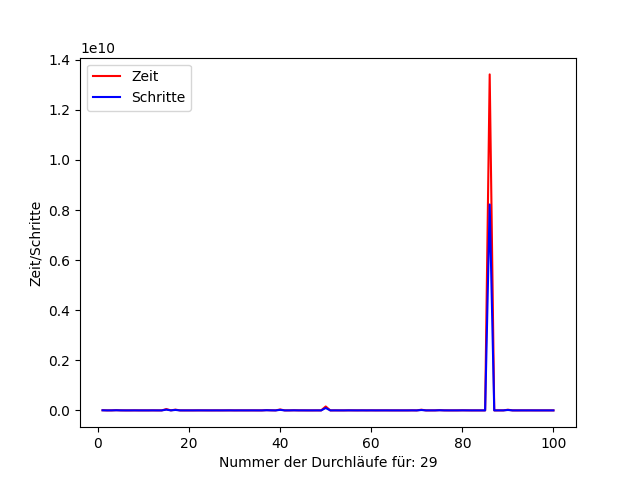
\includegraphics[scale=.5]{29.png}
\caption{Plot Durchlauf 29, erster Versuch}
\label{fig:Plot 29}
\end{figure}

Bei der Betrachtung der Lösung eines einzelnen Labyrinths fällt auf, dass die Zeit und Schritte, welche benötigt wurden um dieses Labyrinth zu lösen, bis auf ein paar Ausreißer, in einem gewissen Bereich gleich nah aneinander liegen.
Ein hervorragendes Beispiel dafür ist der Durchlauf 29, zu sehen in Abbildung \ref{fig:Plot 29}, aus dem ersten Versuch.
Dort ist nur ein Ausreißer deutlich zu erkenne, ansonsten liegen die Werte nah bei einander.

\begin{figure}[h]
\centering
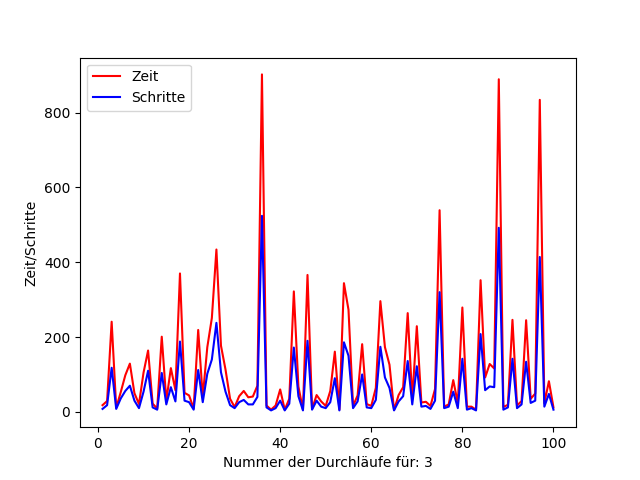
\includegraphics[scale=.5]{3.png}
\caption{Plot Durchlauf 3, erster Versuch}
\label{fig:Plot 3}
\end{figure}

Zu beachten ist jedoch, dass die Werte nicht durchgehend die selben sind, abgesehen von den zuvor erwähnten Ausreißern, wie man es aus Abbildung \ref{fig:Plot 29} annehmen kann.
Dass die Werte unterschiedlich sind und doch in der Nähe der anderen Werte liegen sieht man in Abbildung \ref{fig:Plot 3}, wo der Durchlauf 3 des ersten Versuches zu sehen ist.

Nimmt man nun den Durchschnitt der Zeit und Schritte jeder Labyrinthsgröße und ermittelt dafür jeweils den Durchschnitt, so kann man anhand eines Plots ablesen, wie sich die benötigten Schritte und Zeit im Verhältnis zur Labyrinthsgröße verhalten.

\begin{figure}[h]
	\centering
	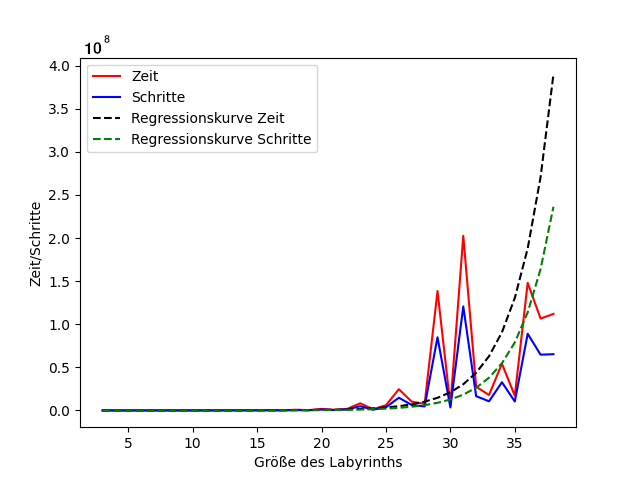
\includegraphics[scale=.5]{v1Aus.png}
	\caption{erster Versuch}
	\label{fig:Plot v1}
\end{figure}
 
In Abbildung \ref{fig:Plot v1} ist der erste Versuch abgebildet.
In diesem ist zu erkennen, dass sich bis Labyrinthgröße 22 keine starke Veränderung der benötigten Zeit oder Schritte einstellt.
Bei Labyrinthgröße 23 ist der erste kleine Ausschlag zu erkennen und bei Labyrinthgröße 29 und 31 befinden sich die ersten beiden starken Ausschläge, wobei sich Größe 30 wieder in der Nähe der Größen bis 22 befindet.
Anschließend findet ein leichter Anstieg statt und ein starker Ausschlag bei Größe 36.

\begin{figure}[t]
	\centering
	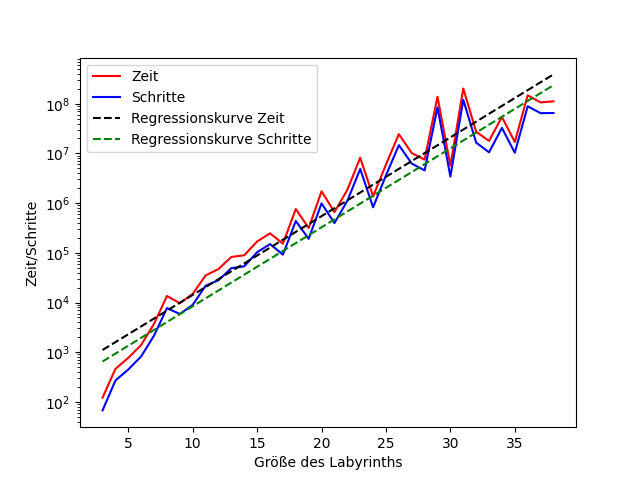
\includegraphics[scale=.5]{v1AusLog.png}
	\caption{erster Versuch, Log-Plot}
	\label{fig:Plot v1Log}
\end{figure}

Wird nun eine Regressionskurve eingefügt, so ist zu erkennen, dass der Anstieg einer Exponentialfunktion ähnelt.
Im logarithmischen Plot Abbildung \ref{fig:Plot v1Log} ist dies eindeutig zu sehen, da die Regressionskurve zu einer perfekten Gerade geworden ist.
Somit ist die Regressionskurve eine Exponentialfunktion und die Schritte bzw. Zeit steigen exponentiel.

\begin{figure}[h]
\begin{minipage}{.5\textwidth}
	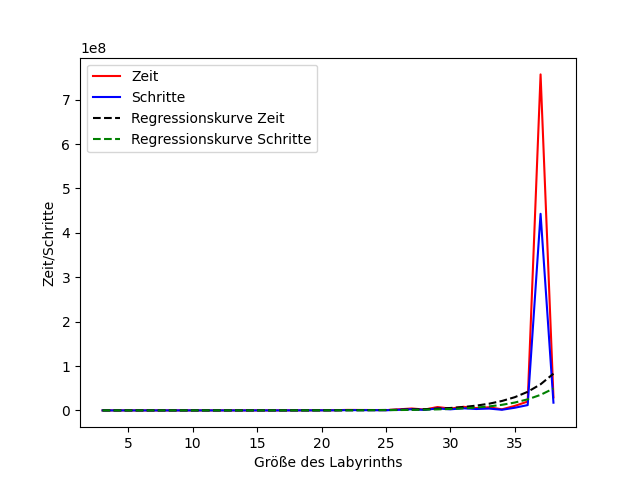
\includegraphics[scale=.45]{v2Aus.png}
	\caption{zweiter Versuch}
	\label{fig:Plot v2}
\end{minipage}
\begin{minipage}{.5\textwidth}
	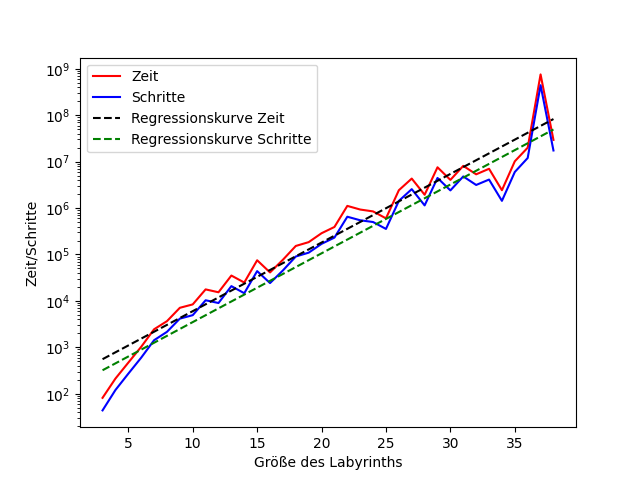
\includegraphics[scale=.45]{v2AusLog.png}
	\caption{zweiter Versuch, Log-Plot}
	\label{fig:Plot v2Log}
\end{minipage}
\end{figure}

Die gleiche Betrachtung ist ebenfalls auf den zweiten Versuch, Abbildung \ref{fig:Plot v2} anwendbar, hier ist auffällig, dass es nur einen Ausschlag gibt, welcher auffällt.
Dieser liegt bei Labyrinthgröße 37.
Durch Einfügen einer Regressionkurve sieht man in diesem Plot ebenfalls den Ansatz exponentielem Wachstums, welche sich in Abbildung \ref{fig:Plot v2Log} anhand der Geraden im logarithmischen Plot bestätigen lässt.

\bigskip

Betrachtet man nun den Anstieg der Exponentialfunktionen in Abbildung \ref{fig:Plot v1} und Abbildung \ref{fig:Plot v2} so fällt auf, dass der zweite Versuch, wo der Käfer nur in drei Richtung laufen kann, einen weniger starken Anstieg hat, als der Käfer im ersten Versuch, der in alle vier Richtungen laufen kann.
Dies ist der Fall obwohl der Käfer im zweiten Versuch mehr Schritte machen muss um Rückwärts zu laufen.
Begründen lässt es sich damit, dass es dem Käfer damit auch schwerer fällt seinen Weg wieder rückwärts zu gehen, da dies nur passiert, wenn entweder rückwärts der einzige Weg ist, er als Ausgang in die Richtung guckt, welche rückwärts ist, er in der Routine vorwärts, rechts oder vorwärts, rechts, links den weg Rückwärts beschreitet.
Also ist es dem Käfer nur in vier Fällen möglich rückwärts zu laufen, während der Käfer aus dem ersten Versuch in folgen Fällen rückwärts laufen kann.
In vier Fällen, wenn er in einer Sackgasse ist, in drei Fällen wenn ein Weg hinter ihm ist und einer wo anders, in zwei Fällen wenn ein Weg hinter ihm und zwei Wege vor ihm sind und in einem Fall wen alle Wege offen sind.
Somit ist es dem Käfer in 4 Fällen möglich rückwärts zu gehen.
Folglich kann der Käfer aus dem ersten Versuch potenyiel vier mal so oft seinen Weg wieder zurück gehen als der Käfer aus Versuch zwei.
Es ist aber nur nötig rückwärts zu gehen, wenn der Käfer in einer Sackgasse gelandet ist.
Somit ist der Käfer aus dem zweiten Versuch vier mal schneller als der Käfer aus dem ersten Versuch.
Dies ist ebenfalls aus den Graphen ablesbar, da in Abbildung \ref{fig:Plot v1} die Regressionskurve bei etwa $4 \cdot 10^8$ und in Abbildung \ref{fig:Plot v2} bei etwa $1 \cdot 10^8$ endet.
Zur Prüfung wird ebenfalls der Punkt betrachtet, bei welchem in Abbildung \ref{fig:Plot v2} die Regressionskurve bei etwa $0,5 \cdot 10^8$ sich befindet, welcher bei 36 liegt.
Anschließend wird dieser Wert vervierfacht, was 2 ergibt und in Abbildung \ref{fig:Plot v1} bei x gleich 36 der Wert der Regressionskurve abgelesen, welcher etwa 2 beträgt.

\section{Fehlerbetrachtung}

Auf Grund eines kleinen Datensets sind die Daten fehlerbehaftet, da ein einziger Durchlauf, in dem die Zahl der Schritte deutlich höher ist alles alle anderen den Durchschnitt hochzieht.
Als Beispiel ist Abbildung \ref{fig:Plot 29} anzuführen, dort ist erkennbar, dass bis auf einen Fall die Zeiten an nährend gleich sind.
Mit diesem Ausfall liegt der Durchschnitt jedoch über diesen Zeiten.
Dem könnte mit einer höheren Anzahl an Werten entgegen gewirkt werden.
Ebenfalls ist in dem zweiten Versuch, siehe Abbildung \ref{fig:Plot v2}, zu erkennen, dass der exponentiele Anstieg ebenfalls durch einen Ausfall der Messwerte entsteht.
Um sicherzustellen, dass der Anstieg exoponentiel ist, müssten weitere Werte für größere Labyrinthe erhoben werden.

\section{Fazit}

In dem Experiment, wurde ein Labyrinth erzeugt, welches immer lösbar ist und nur einen richtigen Weg besitzt.
Durch dieses Labyrinth wurde ein Käfer geschickt, welcher im Uhrzeigersinn geprüft hat, ob sich an dieser Stelle eine Wand befand und wenn nicht sich auf diesen Punkt bewegt hat, dabei wurde die erste Wand welche geprüft wird zufällig ausgewählt.
Im zweiten Versuch war es dem Käfer nicht möglich direkt rückwärts zu laufen, um dies zu tun musste er sich um 90° drehen.
Dabei wurden die Anzahl der Schritte und die Anzahl der erfolgten Aktionen, als Zeit definiert, gespeichert.


\bigskip

Nach Betrachtung der Daten sind folgende Erkenntnisse aufgetreten.
Es viel auf, das obwohl die Richtung, in welche sich der Käfer bewegt, zufällig gewählt wurden, der Käfer unterschiedliche Labyrinthe von der selben Größe in etwa der selben Zeit und Schrittzahl löst.
Des weiteren wurde festgestellt, dass bei Betrachtung der benötigten Zeit und Schritte, über die verschiedenen Labyrinthgrößen, ein exponentieler Anstieg zu erkennen ist.
Dabei ist aufgefallen, das der Anstieg während des ersten Versuchs ungefähr vier mal so groß ist, wie während des zweiten Versuchs, was darauf zurück zu führen ist, dass der Käfer während des zweiten Versuch aufgrund seiner Einschränkung nicht rückwärts laufen zu können ohne eine Drehung diese Bewegung weniger oft ausführte.
Dadurch bewegte er sich weniger häufig auf Felder, auf welchen er sich vorher befand.
Daraus entsteht die Erkenntnis, dass es schneller ist ein Labyrinth zu lösen, in dem nur zurückgegangen wird, wenn eine Sackgasse erreicht wird.

\bigskip

Probleme während der Durchführung des Experiments, waren die Sicherstellung der Lösbarkeit des Labyrinths sowie das Speichern der Daten.
Beim Speichern der Daten war es geplant ebenfalls den genauen Pfad des Käfers zu speichern.
Dies erwies sich jedoch als nicht möglich, da mir drei Daten der Labyrinthgröße 15, 17 und 18 eine Speichermenge von ca. 154Gb erreicht wurde, was ca 17\% des gesamt verfügbaren Speichers entsprach.
Ebenfalls geplant war es bis zu einer Labyrinthgröße von 50 zu testen.
Dies war ebenfalls nicht möglich, da nach Labyrinthgröße 38 im ersten Versuch und Lagyrinthgröße 41 im zweiten Versuch die für das Programm verfügbaren CPU Kerne zu 100\% genutzt waren und das Programm nicht weiter lief.
Das letzte Problem war, das durch einen Fehler im Code die Daten 100 mal in der selben Datei gespeichert wurden anstatt einmal.

\newpage

\printbibliography 






\end{document}
